The goal of query 2 is to identify outliers that consume significantly higher amount of energy compared with the average consumption computed globally.
A plug is counted as an outlier if median load of the plug is more than the median load of all the plugs in the system for a given sliding window (1 hr or 24 hrs).
We need to produce an output event when the percentage of such plugs in a house changes.

\subsection{Architecture}
To evaluate Query 2, we have to compute global median i.e. median of all the data of all the plugs in the system acquired in a given sliding window of length 1 hr and 24 hrs. Then, we compute percentage of outlier plugs every time we receive a new event using plug medians. The frequent comparison of locally computed data with global data enforces a single node solution for all the houses in case of Query 2.

There are two processes in the system residing on different nodes. The broker process reads data from a file and sends events to the Q2 process. Q2 keeps a linked list of all the events of last 24 hrs in the order they have been received. It also keeps instances of Sliding Median Container (SlidingMc) class in order to compute various medians and S Container (SCont) class for the purpose of finding the number of outliers in every house.

\begin{figure}[h]
\begin{center}
\begin{tikzpicture}[scale=1, transform shape, shorten >=1pt, node distance=0.8cm,auto]
\tikzstyle{every state}=[draw=black!70, rectangle, very thick, fill=black!20]
\node[state] (I1) {$T_0$};
\node[state] (I2) [right of=I1] {};
\node[state] (I3) [right of=I2] {};
\node[state] (I4) [right of=I3] {$$};
\node[state] (I5) [right of=I4] {$T_W$};
\node[state] (I6) [right of=I5] {$$};
\node[state] (I7) [right of=I6] {$$};
\node[state] (I8) [right of=I7] {$$};
\node[state] (I9) [right of=I8] {$T_E$};

\draw [decorate,decoration={brace,amplitude=10pt,mirror,raise=10pt},yshift=0pt] (I5.center) -- (I9.center);
\node (text) at (5,-1) {Window W};
\end{tikzpicture}
\vspace*{-0.4cm}
\caption{Linked List in Q2 process \label{fig:linked_list}}
\end{center}
\end{figure}
\vspace*{-0.3cm}

Let's assume an event \textit{E} is received by the Q2 process from the broker process with timestamp \textit{$T_E$}.
Let's also assume the window size to be \textit{W} which can be either 1 hr or 24 hrs.
\textit{$T_W$} is the minimum timestamp which exists in the window of length \textit{W} terminating with the event E as shown in the Figure \ref{fig:linked_list}. Note that there may be multiple events with the timestamp $T_W$ in the window. In such a case, we choose the left most event with the same timestamp $T_W$ in the linked list. Also, if the data corresponding to the timestamp $\tau = (T_E - W +1)$ is missing, then $T_W$ will be the first timestamp bigger than $\tau$ for which event for any plug in the system is present. Now, the algorithm proceeds as follows.
We shift the left end of the window one event, keeping the right end fixed. We delete the oldest event from the median container of the corresponding plug and the global median container.
Now, we compute new median of the plug and insert the new median into the S container of the house.
S container is, then, queried to find out whether the percentage of outliers for a given house has changed after the shift. We output an event if any of the percentage for any house has changed.
On the other hand, if the global median doesn't change, we only check the percentage number of outliers for the house corresponding to the deleted event.

We stop when the leftmost event in the window has the timestamp $T_W$. In the last slide, before computing any medians, we also insert the newly received event $E$ into the global median container and the median container of the plug of the event E. Rest of the computation remains same. To avoid redundant storage of the data, we keep the linked list only for 24 hrs sliding window, and keep a pointer to the first event of the 1 hr window in the same linked list.

\subsection{Median Algorithm}
In query 2, we have to compute the median of large amounts of data frequently. A trade off exists between the computational complexity and accuracy of the median so derived. The basic idea\footnote{The Algorithm is inspired from discussions on \url{http://stackoverflow.com/questions/638030}} is to construct a histogram of the data using fixed number of bins (M-1). We sort the first M distinct values inserted into the container and use them in order to build up the (M-1) bins. Every bin is associated with a frequency denoting the frequency of the data greater than equal to $i^{th}$ lowest value (including) but less than $(i+1)^{th}$ lowest values (excluding) among M inserted value into the container. We also store the index of the bin containing the median after an insertion or deletion is performed, cumulative sum of the frequencies upto and including the bin in which median resides and the total number of values inserted into the container. These numbers are used in order to quickly find the median of all values present in the system.

To adapt the histogram of newly coming data, the bin configuration is changed dynamically. A bin is split into two bins if it becomes too full and deleted if it becomes empty. If number of bins are higher than the maximum allowed number of bins, we merge 2 bins. The insert and delete operation takes O(M) time in the worst case whereas getMedian is a constant order operation.

We did 1000 experiments to find the Relative Error for median container, each inserting 50000 random values into the container. The CDF is plotted in the Figure \ref{fig:relative_error}. It can be observed that there is very low relative error due to the approximation. We also did several tuning experiments and found that bin size greater than 1200 gives lowest error. Hence we use 1200 as bin size in the implementation of Query 2.

\begin{figure}[h]
\begin{center}
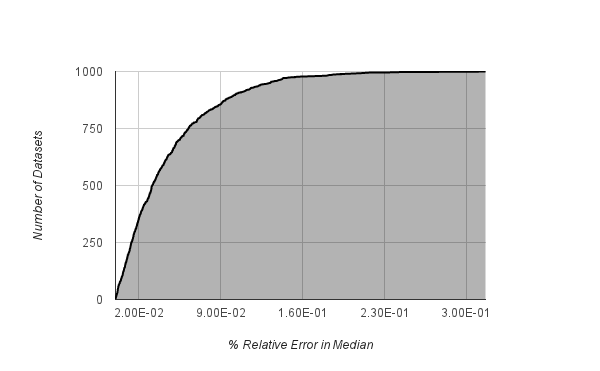
\includegraphics[scale=0.5]{img/relative_error}
\vspace*{-0.3cm}
\caption{CDF of Relative Error \label{fig:relative_error}}
\end{center}
\vspace*{-0.7cm}
\end{figure}

\subsection{S Container}
$S$ Container is used to efficiently compute number of plugs in a house having higher median load than the global median load (\textit{getNumOfLargeNum}() function). The challenge in implementing $S$ Container is that we don't know number of plugs in a house before hand. Hence, we had to use a map (key-value storage) in order to store the data but that leads to O(K) complexity of the \textit{getNumOfLargeNum} operation where K is the total number of plugs in a house. We avoided this by using an array and stored all the data in sorted order with key being the plug median. When a new value is to be inserted, we require the old plug median in order to search the location of the plug data in the array. As soon as we find the location, we replace the new median with the old median and modify the location such that the array is sorted again.

The asymptotic complexity of this is also O(K) but in the given scenario, a momentous change in median values are unlikely. Very little movement of data, therefore, will be required while sorting the array after an insertion is performed. On the other hand, \textit{getNumOfLargeNum} operation will always be cheaper than $\log(K)$.
 
\subsection{Experimental Evaluation}
We used the same setup as we used in case of Query 1. The broker process is executed on one virtual machine and Q2 process is executed on another virtual machine in the same cluster. We are able to achieve a constant average throughput of 480 thousand events per sec as shown in Figure \ref{fig:q2_throughput}. Because there is only one Q2 process computing all the percentage values, throughput doesn't change significantly in terms of input events/sec as the number of house increases. The utilization level in case of Q2 process is always close to 100\%.

\begin{figure}[h]
\begin{center}
	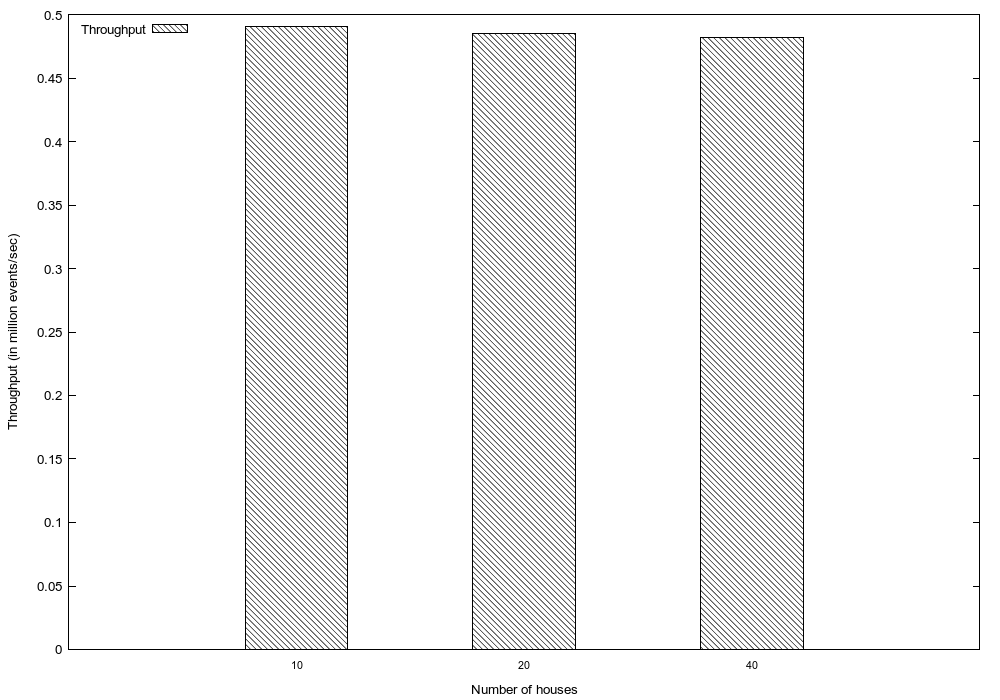
\includegraphics[width=0.4\textwidth]{img/q2_throughput}
	\vspace*{-0.4cm}
	\caption{Throughput vs No.
of Houses (Query 2) \label{fig:q2_throughput}}
\end{center}
\vspace*{-0.5cm}
\end{figure}

Latency corresponding to an output event, in case of Query 2, is defined as the amount of time taken to output event after the corresponding input event is received.
Note that one input event may result in more than one output events and latency of the events output later will be higher. Latency graph for Query 2 is shown in Figure \ref{fig:q2_latency}. 90\% for 10 houses is higher because of biased distribution of data with respect to house.
Houses 0-9 have more amount of data and the number of output events, therefore, will be more for every input event. In such a case, the events output later will have higher latency values.

\begin{figure}[h]
\begin{center}
	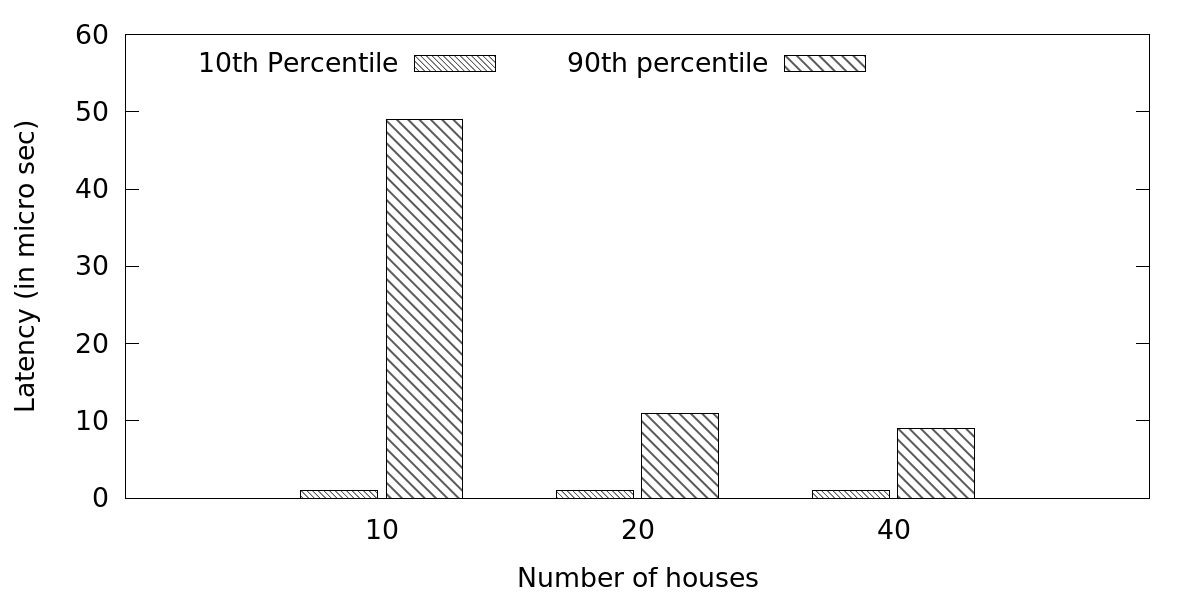
\includegraphics[width=0.4\textwidth]{img/q2_latency}
	\vspace*{-0.3cm}
	\caption{Latency vs No.
of Houses (Query 2) \label{fig:q2_latency}}
\end{center}
\vspace*{-0.5cm}
\end{figure}
